	\chapter{Modelling the Detection of \ac{EWFO}}
	\label{sec:object_detection}
	
	Object Detection can be described by two individual goals: the description of what kind of object is seen (Classification), as well as where it is seen (Localization). Hence, an Object Detection pipeline transforms the raw image to a set of one or more areas and corresponding class labels. Images are high dimensional signals that can contain redundant and task irrelevant information. As the performance of most machine learning models decreases when the feature space becomes too large (curse of dimensionality), Computer Vision pipelines usually apply a feature extraction stage, before the actual prediction is done. An overview is displayed in \Cref{fig:obj_pipeline}.
	
	\begin{figure}[hbtp]
		
		\centering
		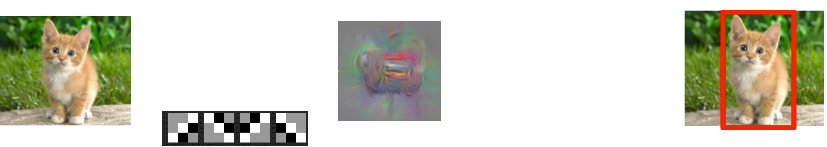
\includegraphics[width=\linewidth]{fig/ObjectDetection}
		\caption{Object Detection Pipeline.where $B_n$ describes an area, $C_1$ a class label, $I$ the image and $f$ the object detection function.}
		\label{fig:obj_pipeline}
	\end{figure}
	\begin{enumerate}
	\item The feature extraction stage extracts task relevant information from the image and infers an internal, more abstract representation that is usually of lower dimension.
	
	\item The classification/localization stage produces the final output based on this representation. 
	
	\end{enumerate}

	An efficient feature extraction pipeline is thereby crucial for the success of an Object Detection pipeline. If the inferred representation is clearly separable, a simple classification stage can distinguish between classes. On the other hand even a flexible classifier struggles with a highly overlapping feature space. Hence, Feature Engineering, the design of feature extractors is a highly investigated field in Computer Vision. Methods range from supervised and unsupervised Machine Learning techniques to conducting domain experts and trying to include their expert knowledge into the pipeline. In practical Computer Vision problems this often results in the cumbersome design of feature extractors for the application. Moreover, it requires domain knowledge and it is questionable whether the features designed for one task are easily transferable to other tasks. Finally, it results in a pipeline where each step needs to be optimized individually.
	
	In recent years Deep Learning based models achieved big advances in the task of Object Detection. In contrast to their traditional counter parts, these models combine Feature Extraction and Classification/Localization stage in one model. The whole pipeline is then optimized given the task and the raw image. This omits the often cumbersome work of designing feature extractors and object models. Furthermore, it has been shown that Deep Learning based features generalize well between different Computer Vision tasks \cite{Razavian}. Finally, the modular architecture of Deep Learning models allows to trade-off computational costs and model performance.
	
	However, their superior performance comes with several drawbacks. First of all, large amounts of annotated examples are required in order to train the vast amount of parameters present in Deep Learning models. Furthermore, the computational costs during training and inference are high. Only faster and tailored processing units like \acp{GPU} enable the practical application of Deep Learning models. Finally, the presentation learned by the model is not transparent. Hence, the process that leads to the decision of a Computer Vision system can usually not be understand by a human. Also, there is no guarantee that the learned representation is not highly redundant. This is particularly problematic for devices with time constraints and limited computational resources like \acp{MAV}.
	
	This work investigates the detection of \acp{EWFO} on \ac{MAV}. \acp{EWFO} consist of simple shapes but are largely occupied by background. Hence, other objects of interest and/or distractors can appear in this area. Furthermore, sensor and lens properties as well as motion noise can have large impact on the appearance of \acp{EWFO} in the image. This makes the design of an appropriate feature extractor a non-trivial task. Deep Learning would allow to learn a feature extractor and object model given data and the task.
	
	This work address the design of a Deep Learning model for the task of \ac{EWFO}-Detection.
	
	The relevant research question of this chapter is stated as follows:\\
	\textbf{How can a detection model represent \acp{EWFO}?}
	
	\begin{enumerate}
		\item[\textbf{RQ2.1}] Can state-of-the art models represent an \ac{EWFO}?
		\item[\textbf{RQ2.2}] What is the representation a state-of-the-art model learns for the Detection of \acp{EWFO}?
		\item[\textbf{RQ2.3}] Can the insights be used to create a more suitable model for the Detection \ac{EWFO}?
	\end{enumerate}

	The first question will be answered by analysing the performance of state of the art model on the detection of \acp{EWFO}. RQ2.2 will be answered by conduction a sensitivity analysis on the trained model and visualizing the internal representation. RQ2.3 will be answered by refactoring the model architecture and examining whether the performance can be improved or weights can be removed.

	The rest of the chapter is organized as follows: \Cref{sec:object_detection:related} discusses relevant related work. \Cref{sec:object_detection:approach} describes the methodology of this work. \Cref{sec:object_detection:hypothesis} formulates several hypotheses to be investigated. \Cref{sec:object_detection:experiments} outlines the experiments conducted to evaluate the formulated hypotheses. \Cref{sec:object_detection:results} describes the obtained results. \Cref{sec:object_detection:discussion} discusses the results. \Cref{sec:object_detection:conclusion} answers the research question and formulates a conclusion.


	\section{Related Work}
	\label{sec:object_detection:related}
	The existing methods can broadly be grouped in three groups. Those are more traditional approaches without \acp{CNN}-based feature extraction, two-stage detectors and one-stage detectors.
	
	\subsection{Traditional Methods}
	
	One of the first object detection methods was \cite{Viola2004} that used simple filters inspired by Haar-basis functions as a feature extractor for human face detection. The image was processed in a cascade of classifiers that assigned the label "face" or "background" to image patches. The output of the first stages were further classified when going deeper in the cascade. The processing of one image patch stopped, when a classifier assigned the label "background". Although being very fast the Haar-based feature extraction is not very robust towards rotation-, scale- or shape-variations \todo{quote}. 
	
	A more robust feature extractor was proposed by \cite{Dalal} and \cite{Lowe2004} for pedestrian detection. A local (normalized) histogram of gradients is computed for a fixed window size. 

	Previously mentioned methods modelled objects as one instance. This prove to be sensitive towards part occlusions or large deformations. Deformable part models detect object parts individually and combine them. Thus a feature extractor can still give a high response when even only object parts are visible or they are arranged in a way untypical to the training set.
	
	Guido proposes a neural network to learn an attention model.
	
	X propose a recurrent neural network architecture to model the attention process.
	
	\todo{discussion traditional features}
	
	\subsection{\acp{CNN}-based Feature Extraction}
	
	In recent years \acp{CNN} emerged from Deep Learning research and became a popular feature extractor. \acp{CNN} can be seen as small neural networks that are applied locally on image patches in sliding window fashion. The outputs of the initial local operations (first layer) are further processed by higher layers until the desired output size is reached. The model parameters (weights) are trained using a Loss function and the back-propagation algorithm.
	
	The modular structure of \acp{CNN} allow to create highly non-linear models that can represent any function. However, this flexibility also introduces the challenge of choosing a suitable architecture. On a fundamental level design parameters can be summarized in depth, width and kernel size. 
	
	\Cref{fig:model_design} displays these parameters and introduces additional terminology necessary for the remaining parts of this chapter. The \textit{kernel size} $\textbf{k}$ determines the spatial size of a kernel and therefore how big the patch is, the convolution is applied on. A layer usually contains multiple filters that are applied on its input. The amount of filters is also referred to as \textit{width} $w$. The filters are applied in sliding window fashion which introduces the step size ( \textit{strides} $\mathbf{s}$) as an additional parameter. The output of each convolution is concatenated and processed by the next layer. The amount of layers is also referred to as \textit{depth}. In the image also the \textit{receptive field} of a filter is visualized. This describes the image patch that is related to a certain feature response. The filter of the first layer (green) has a receptive field corresponding to its kernel size. The filter of the second layer (blue) combines the responses of the filters of the first layer at multiple spatial locations an thus has an increased receptive field.
	
	\begin{figure}[hbtp]
		\centering
		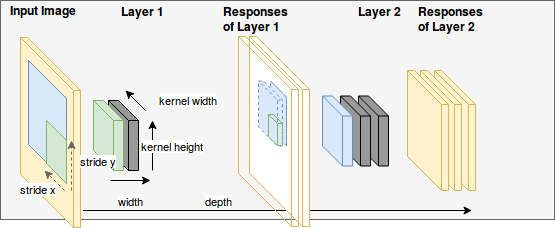
\includegraphics[width=0.8\textwidth]{fig/model_design}
		\label{fig:model_design}
		\caption{Example Architecture of a \ac{CNN}}
	\end{figure}
	
	Among these parameters depth is considered one of the preliminary parameters to improve performance \cite{He}. \citeauthor{Simonyan2014} \cite{Simonyan2014} achieve first places in the 2014 ImageNet Classification challenge using a network that only contained filters of size 3-by-3 but up to 19 layers. \citeauthor{Szegedy2014} \cite{Szegedy2014} achieve similar performance using a network with 22 layers. The proposed network included a \textit{Inception}-module, an architectural element that allows deeper networks at a constant computational budget. 
	
	An issue that prevented training even deeper networks is the \textit{vanishing gradient problem}. As the gradient distributes while flowing through the vast amount of nodes its magnitude gets very small. Hence, the training becomes slow and the risk of converging in a local minima increases. This was addressed by \citeauthor{He2015} \cite{He2015} who propose the use of residual connections. Instead of propagating the gradient from the last to the first layer these connections allow the gradient to flow directly into all layers. This circumvents the vanishing gradient problem. The use of residual connections allowed to train a network 101 layers and improved on state of the art at that time.
	
	However, later work by \citeauthor{Zagoruyko2016} \cite{Zagoruyko2016} shows how residual networks do not behave like a single deep model but more like an ensemble of more shallow networks. Moreover, the study shows that similar performance can be achieved by particularly wide networks and residual connections. Being of similar performance the proposed \acp{WRN} are computationally more efficient to execute.
	
	While wide residual networks can achieve similar performance to deep residual networks with reduced inference time the computational requirements are still large. This work addresses the detection of \ac{EWFO} with very limited resources. Hence, a network in which the vanishing gradient problem would appear is likely to be already too computationally expensive to be applied on a \ac{MAV}.
	
	Instead the work focuses on much smaller networks that are fast to execute. Execution time is also the motivation for \acp{FCN}. Instead of using a fully connected layer in the last stage, these network only apply local operations. This saves many computations in the last layer and enables the application of models on various input sizes.
	
	However, \ac{FCN} in combination with a small amount of layers introduce a limited receptive field. A way to increase the receptive field without increasing the number of computations was proposed by Atrous/Dilated convolutions consist of a sparse kernel thereby increasing the receptive field of a filter without increasing complexity or number of computations \todoref{Atrous}.
	
	Despite a large amount of research conducted in finding suitable architectures there has not yet been a single way that always achieves a goal. It has been shown how models with a large amount of parameters combined with huge training data perform well on various vision tasks and objects. However, there is no guarantee that the found representation is also the most suitable/efficient one. The research resulted in a collection of rules an best practices that need to be considered with the task at hand. This work investigates the design of a \ac{CNN} for the detection of \ac{EWFO}.
	
	\subsection{\ac{CNN}-based Object Detection}
	
	\acp{CNN}-based feature extraction is employed in various approaches to Object Detection. 	

	\citeauthor{Girshick2013} \cite{Girshick2013} use the Selective Search algorithm \cite{Uijlings2013} to extract object candidates from an image and classify each region with a \ac{CNN}. However, this requires to run the whole network at various scales and overlapping locations. Hence, the approach contains a lot of redundant operations and is computationally intense.
	
	\citeauthor{Ren} \cite{Ren} use a \ac{RPN} to propose regions that likely contain an object. In order to define the proposal task as a regression problem, the approach introduces so called \textit{anchor boxes}(also \textit{prior boxes}, \textit{default boxes}). These are boxes of predefined size and location. The model predicts class probabilities and coordinate offsets for each of these boxes. Hence, a certain set of output nodes is responsible for a particular box. If during training a ground truth box has sufficient overlap with a certain box the corresponding output nodes are assigned "responsible" to predict that object. That means the loss is only propagated via those nodes. 
	
	\Cref{fig:anchors} illustrates the concept. The anchor boxes are displayed as dashed lines while the ground truth is displayed solid. The ground truth box in blue has sufficient overlap with two anchor boxes. Hence, these two sets of output nodes take part in the loss calculation. In the example each of these sets predicts coordinate offsets $\Delta(cx, cy, w,h)$ and class probabilities $c_1 .. c_p$.
	
\begin{figure}[hbtp]
	
	\centering
	\captionsetup{justification=raggedright,singlelinecheck=false}
	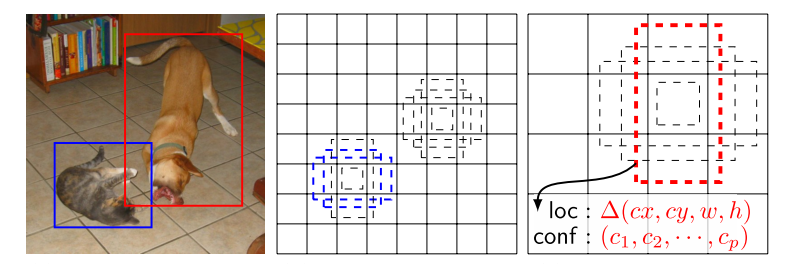
\includegraphics[width=0.8\linewidth]{fig/anchors}
	\caption{Visualization of the anchor box concept \cite{Liu}.}
	\label{fig:anchors}
	
\end{figure}

For the classification stage an \ac{SVM}-classifier is used. The classifier is trained on the image patches extracted by the first stage. \acp{RPN} enabled to propose multiple candidate regions with a single inference of the network. Thus, the expensive feature extraction stage is run only once which results in a significant speed up \todo{how much?}. A drawback is the fact that individual stages of the method have to be optimized individually. Furthermore, the training requires to store large amounts of extracted patches on the hard drive.

In the follow up work \cite{Ren} propose the \textit{ROI}-pooling layer. The layer uses spatial pyramid pooling in order to resize region proposals to a fixed size. This enabled the end-to-end training of the two-stage detection pipeline. \todo{And resulted in?}
	
Another end-to-end pipeline was published by \citeauthor{Redmon} \cite{Redmon}. In contrast to aforementioned approaches, the network performs Classification and Localization in a single pass. The task is formulated by dividing the input image in a fixed grid and predicting $C$ class probabilities for each grid cell. Additional $5*B$ output nodes predict $B$ set of bounding box coordinates and $B$ object probabilities for each cell. \todo{what is good and bad?}

\citeauthor{Liu} propose \ac{SSD} \cite{Liu}, one stage detector using the concept of aforementioned anchor boxes. Instead of only predicting an object score for each anchor box, the model also predicts class probabilities. Another novelty in this approach is the use of multiple predictor layers for various scales. The network does not only use its final layer for prediction but also intermediate representations. Assuming that the lower layers preserve more fine grained features, early output nodes are trained on smaller objects while later output nodes focus on predicting larger scale objects.

Follow up work of \citeauthor{Redmon}\cite{Redmon, Redmona} also included the concept of anchor boxes and prediction layers at multiple scales, making \ac{SSD} and \ac{Yolo} converge to a very similar solution. A novelty in \cite{Redmona} is the use of de-convolution layers for small object prediction. In order to achieve a higher accuracy for small objects the final layers are up-sampled and combined with finer grain features from earlier layers. The aim is to enable a combination of deep semantic features at low spatial resolution with fine grain low level features at high resolution.

Within the framework of \ac{SSD} and \ac{Yolo} several approaches exist that either change the base network or modify layers in between: \cite{ChengchengNing2017} propose propose a more efficient non-max-suppression method as well as to include an inception module in the network architecture to reduce computation while keeping/increasing performance. \cite{Wu} uses \textit{SqueezeNet} as base network and a mixture between the ssd and yolo loss function as training goal. \cite{Xiang} investigates the receptive fields of SSD and tries to incorporate more context, especially on lower feature maps, to increase detection rate for small objects.\cite{Linb} applies the framework for vehicle detection. They use \textit{GoogLeNet} as base network (and investigate several others).\cite{TripathiSanDiego} apply a network very similar to YoloV2 and investigate 8bit quantization of the model to make it runnable on embedded devices.

A common problem of one stage detectors is the imbalance between background and object samples. Most methods upweigh the positive samples and/or use hard negative mining. \cite{Lin} introduces the \textit{Focal Loss} which focuses on sparse positive samples by design.

\todoref{CornerNet}


Each of the described group of methods has strengths and weaknesses. While shallow methods are typically quite fast they require a lot of manual effort and/or are not so accurate. Two-stage detectors on the other hand are quite accurate but their computational requirements are prohibitive for the hardware to be used in this thesis. One-stage detectors offer a compromise between detection accuracy and inference speed. In addition they can be trained end-to-end which requires only little manual engineering. However, the presented methods are still too slow for the hardware used in this thesis.


	

	%			\paragraph{Scalable Object Detection using Deep Neural Networks\cite{Erhan}}
	%			\begin{itemize}
	%				\item[-] Generates number of bounding boxes as object candidates (class agnostic) and confidences for each box
	%				\item[-] For each Bounding Box a classifier is run e.g. DNN
	%				\item[-] Training: If the number of boxes k is larger than the number of objects b, only b boxes are matched while the confidence of the others is minimized
	%				\item[-] Assignment problem $$F_{match}(x,l) = \frac{1}{2}\sum_{i,j}x_{ij}||l_i - g_j||^2_2$$ where $x_ij$ is one if the ith prediction is assigned to the jth ground truth object
	%				\item[-] Confidence: 
	%				$$F_{conf}(x,c) = - \sum_{i,j}x_{ij}*\log(c_i)-\sum_{i}(1-\sum_{j}x_{ij})\log{1-c_j}$$
	%				\item[-] Speed up training by clustering (kmeans) of ground truth and using it as prior (prior matching)
	%				\item[-] Can be defined to output boxes only for a particular class by training the bounding boxes on that class
	%				\item[-] Number of parameters grows linearly with number of classes
	%				\item[-] Authors argue two step process (region proposal + classification) is better
	%				\item[-] Architecture based on AlexNet
	%				\item[-] Predicted boxes are merged using non-maxima surpression
	%				\item[-] One shot(50\%), +2scales (75\%)
	%				\item[-] OverFeat/ Selective Search are faster but much more expensive
	%			\end{itemize}
	



\todoref{Wire detection}


\section{Approach}
\label{sec:object_detection:approach}
	$$
	L({p_i},{t_i}) = \frac{1}{N_{cls}} \sum L_{cls}(p_i,p_i*) + \lambda \frac{1}{N_{reg}} p_i* L_{reg}(t_i,t_i*)
	$$
	
	Where $i$ is an anchor, $p_i$ the predicted probability of the anchor being an object and $t_i$ a vector containing 4 bounding box offsets to the default anchor size. The ground truth label $t_i*$ contains the true coordinates, while $p_i*$ is 1 if the anchor overlaps a ground truth bounding box by some threshold. \todo{Which exact loss functions are used}


Comparing state of the art results shows the superiority of \acp{CNN}-based methods in basically every vision task \todo{elaborate}. Hence, the first hypothesis formulated is that a state of the art object detector should be able to learn the detection task of wire frame objects. 

As the single class case is considered the loss functions of state of the art detectors is simplified to the following:

\todo{text}

Hence, the only difference between X,Y,Z is ...
Therefore the second hypothesis to be evaluated is that there is not a very large difference between the mentioned methods.


The reason to be assumed responsible for the superiority of \acp{CNN}-based methods is the fact that the can learn powerful object representations directly on the task. \todoref{visualizing cnns} show how the model combines simple shapes like edges, corners and blobs to more complex shapes like noses and eyes. For the task of wire-frame object detection there is no such intuitive combination of such higher order shapes. Therefore the second hypothesis formulated is that the deeper levels of a \acp{CNN} are not necessary for the detector.

\section{Hypothesis}

\label{sec:object_detection:hypothesis}
Several hypothesis are formulated and will be examined experimentally:
\begin{enumerate}
	\item[$\mathcal{H}_1$] \textbf{A \acp{CNN} should be able to learn the object detection task.}
	\item[$\mathcal{H}_2$] \textbf{Considering the single class case state of the art methods will learn the same representation}
	\item[$\mathcal{H}_3$] \textbf{For wireframe objects the deeper layers don't learn anything as the object consist of relatively simple shapes.}
	
\end{enumerate}
\newpage
\section{Experiments}

First we show that many weights in an object detector are superflous when detecting single wire frame objects:
1. We train an object detector on a single but complex object and compare the filters to multiple objects
2. We train an object detector on a single wireframe object and compare the filters to the other feature detectors
3. We use the gained insights to prune the network 
4. The pruned network should perform poorly when used on the complex object
4. We analyse the new network in terms of sensitivity towards: occlusion, colour, distance, angle

\section{Results}

\section{Conclusion}